\newSec[DDDModell]{Domänenmodell}{2}

Um Personen der  Rolle \textit{Domänen-Expert*in} vor unnötigen Programmier-Details (Komplexität) zu schützen, wird ein \textit{Domänenmodell} entwickelt. Hier bildet sich lediglich die \textit{inhärente Komplexität} ab.

Im vorliegenden Projekt können grundsätzlich zwei verschieden abgegrenzte Domänenmodelle zugrunde gelegt werden:
\begin{itemize}
\item Ein Modell, welches sich auf die regelungstechnischen Zusammenhänge des Projekts bezieht.
\item Ein Modell, welches die Interaktion mit der Drohne beschreibt.
\end{itemize}

Das Modell in \refImg{fig:DomainMod} begrenzt sich auf die Betrachtung der Regelung einer Drohne. 

\begin{figure}[ht!]
\vspace{0.25cm}
\begin{center}
\fbox{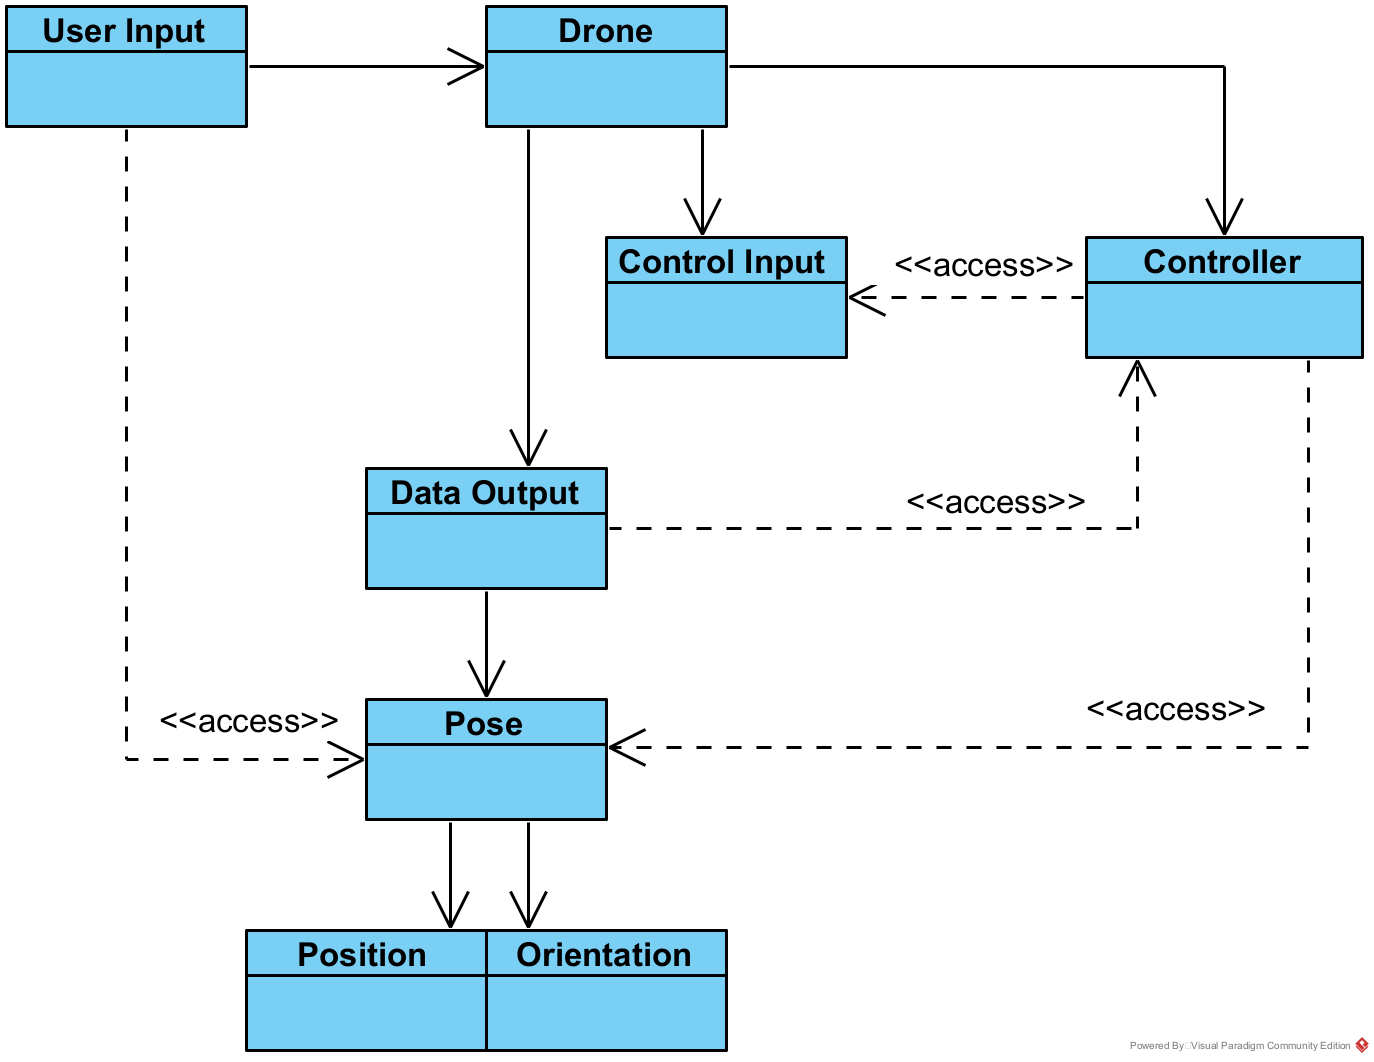
\includegraphics[width=15cm]{Pictures/Domain Modell.png}}
\caption{Domänenmodell des Projekts}
\label{fig:DomainMod}
\end{center}

\vspace{0.25cm}
Die gestrichelten Pfeile deuten eine Nutzung der entsprechenden Klasse an, wobei hier kein Attribut innerhalb der ausgehenden Klasse vorgesehen.
\end{figure}






